\documentclass[12pt]{article}
\usepackage{url, graphicx, epstopdf, amsmath, esint}
\usepackage{physics}

% page layout
\setlength{\topmargin}{-0.25in}
\setlength{\textheight}{9.5in}
\setlength{\headheight}{0in}
\setlength{\headsep}{0in}
\setlength{\parindent}{1.1\baselineskip}
\addtolength{\oddsidemargin}{-0.75in}
\setlength{\marginparwidth}{2in}

% problem formatting
\newcommand{\problemname}{Problem}
\newcounter{problem}
\newcommand{\startproblem}{\paragraph{Problem~\theproblem:}\refstepcounter{problem}}

% words
\newcommand{\foreign}[1]{\textsl{#1}}
\newcommand{\vs}{\foreign{vs}}

% math
\renewcommand{\vec}[1]{\boldsymbol{#1}}
% \newcommand{\dd}{\mathrm{d}} % PROVIDED IN physics PACKAGE
\newcommand{\e}{\mathrm{e}}
% \newcommand{\cross}{\times} % PROVIDED IN physics PACKAGE
% \newcommand{\curl}{\vec{\nabla}\times} % PROVIDED IN physics PACKAGE

% primary units
\newcommand{\rad}{\mathrm{rad}}
\newcommand{\kg}{\mathrm{kg}}
\newcommand{\m}{\mathrm{m}}
\newcommand{\s}{\mathrm{s}}
\newcommand{\A}{\mathrm{A}}

% secondary units
\renewcommand{\deg}{\mathrm{deg}}
\newcommand{\km}{\mathrm{km}}
\newcommand{\cm}{\mathrm{cm}}
\newcommand{\mm}{\mathrm{mm}}
\newcommand{\mum}{\mathrm{\mu m}}
\newcommand{\nm}{\mathrm{nm}}
\newcommand{\ft}{\mathrm{ft}}
\newcommand{\mi}{\mathrm{mi}}
\newcommand{\AU}{\mathrm{AU}}
\newcommand{\ns}{\mathrm{ns}}
\newcommand{\h}{\mathrm{h}}
\newcommand{\yr}{\mathrm{yr}}
\newcommand{\N}{\mathrm{N}}
\newcommand{\J}{\mathrm{J}}
\newcommand{\eV}{\mathrm{eV}}
\newcommand{\MeV}{\mathrm{MeV}}
\newcommand{\W}{\mathrm{W}}
\newcommand{\Pa}{\mathrm{Pa}}
\newcommand{\C}{\mathrm{C}}
\newcommand{\V}{\mathrm{V}}
\newcommand{\ohm}{\mathrm{\Omega}}
\newcommand{\muF}{\mathrm{\mu F}}
\newcommand{\Hz}{\mathrm{Hz}}
\newcommand{\GHz}{\mathrm{GHz}}

% derived units
\newcommand{\mps}{\m\,\s^{-1}}
\newcommand{\mph}{\mi\,\h^{-1}}
\newcommand{\mpss}{\m\,\s^{-2}}
\newcommand{\radps}{\rad\,\s^{-1}}

% random stuff
\sloppy\sloppypar\raggedbottom\frenchspacing\thispagestyle{empty}

\begin{document}

\section*{NYU Physics 2---Problem Set 7}

Due Thursday 2020 April 2 before lecture.

\paragraph{Problem~\theproblem:}\refstepcounter{problem}%
The definition of the electric field $\vec{E}$ and magnetic field
$\vec{B}$ is
\begin{equation}
  \vec{F} = q\,[\vec{E} + \vec{v}\cross\vec{B}]
  \quad .
\end{equation}
Gauss's Law and Ampere's Law are
\begin{equation}
  \oiint\vec{E}\cdot\dd\vec{a} = \frac{Q}{\epsilon_0}
  \quad ;
\end{equation}
\begin{equation}
  \oint\vec{B}\cdot\dd\vec{\ell} = \mu_0\,I
  \quad .
\end{equation}
Use these three equations to figure out the units of the inverse
product $1/(\mu_0\,\epsilon_0)$. What extremely fundamental constant
is this going to be related to?

\textit{Hint:} Gauss's Law has the units of an electric field times an
area. Ampere's Law has the units of a magnetic field times a
length. And the definition of the fields tells you that the units of
the magnetic field differ from the units of the electric field by a
factor of velocity. Does this help?

\paragraph{Problem~\theproblem:}\refstepcounter{problem}%
Use the Biot-Savart Law
\begin{equation}
  \dd\vec{B} = \frac{\mu_0\,I}{4\pi}\,\frac{\dd\vec{\ell}\cross\vec{r}}{|\vec{r}|^3}
\end{equation}
to show that the magnetic field $\vec{B}$ at the center of a circular
ring of radius $R$ carrying current $I$ has magnitude
$(\mu_0\,I)/(2\,R)$. What direction is the field? You might want to
read up on the Biot-Savart methodology for computing a magnetic field
from a current-carrying wire.

\paragraph{Problem~\theproblem:}\refstepcounter{problem}%
Consider a pair of very very long straight wires carrying current $I$,
separated by a distance $2\,a$, connected at their ends by a
semicircular arc of wire of radius $a$ as shown. What is the magnetic
field $\vec{B}$ at the point indicated as $Q$? Give the magnitude and
the direction of the field. Unlike what is shown in the drawing,
the idea is that the straight portions go on for a very long distance;
way way longer than $a$.

\textit{Hint:} You will want to use superposition and symmetry to
solve this one, not the integral!
\marginpar{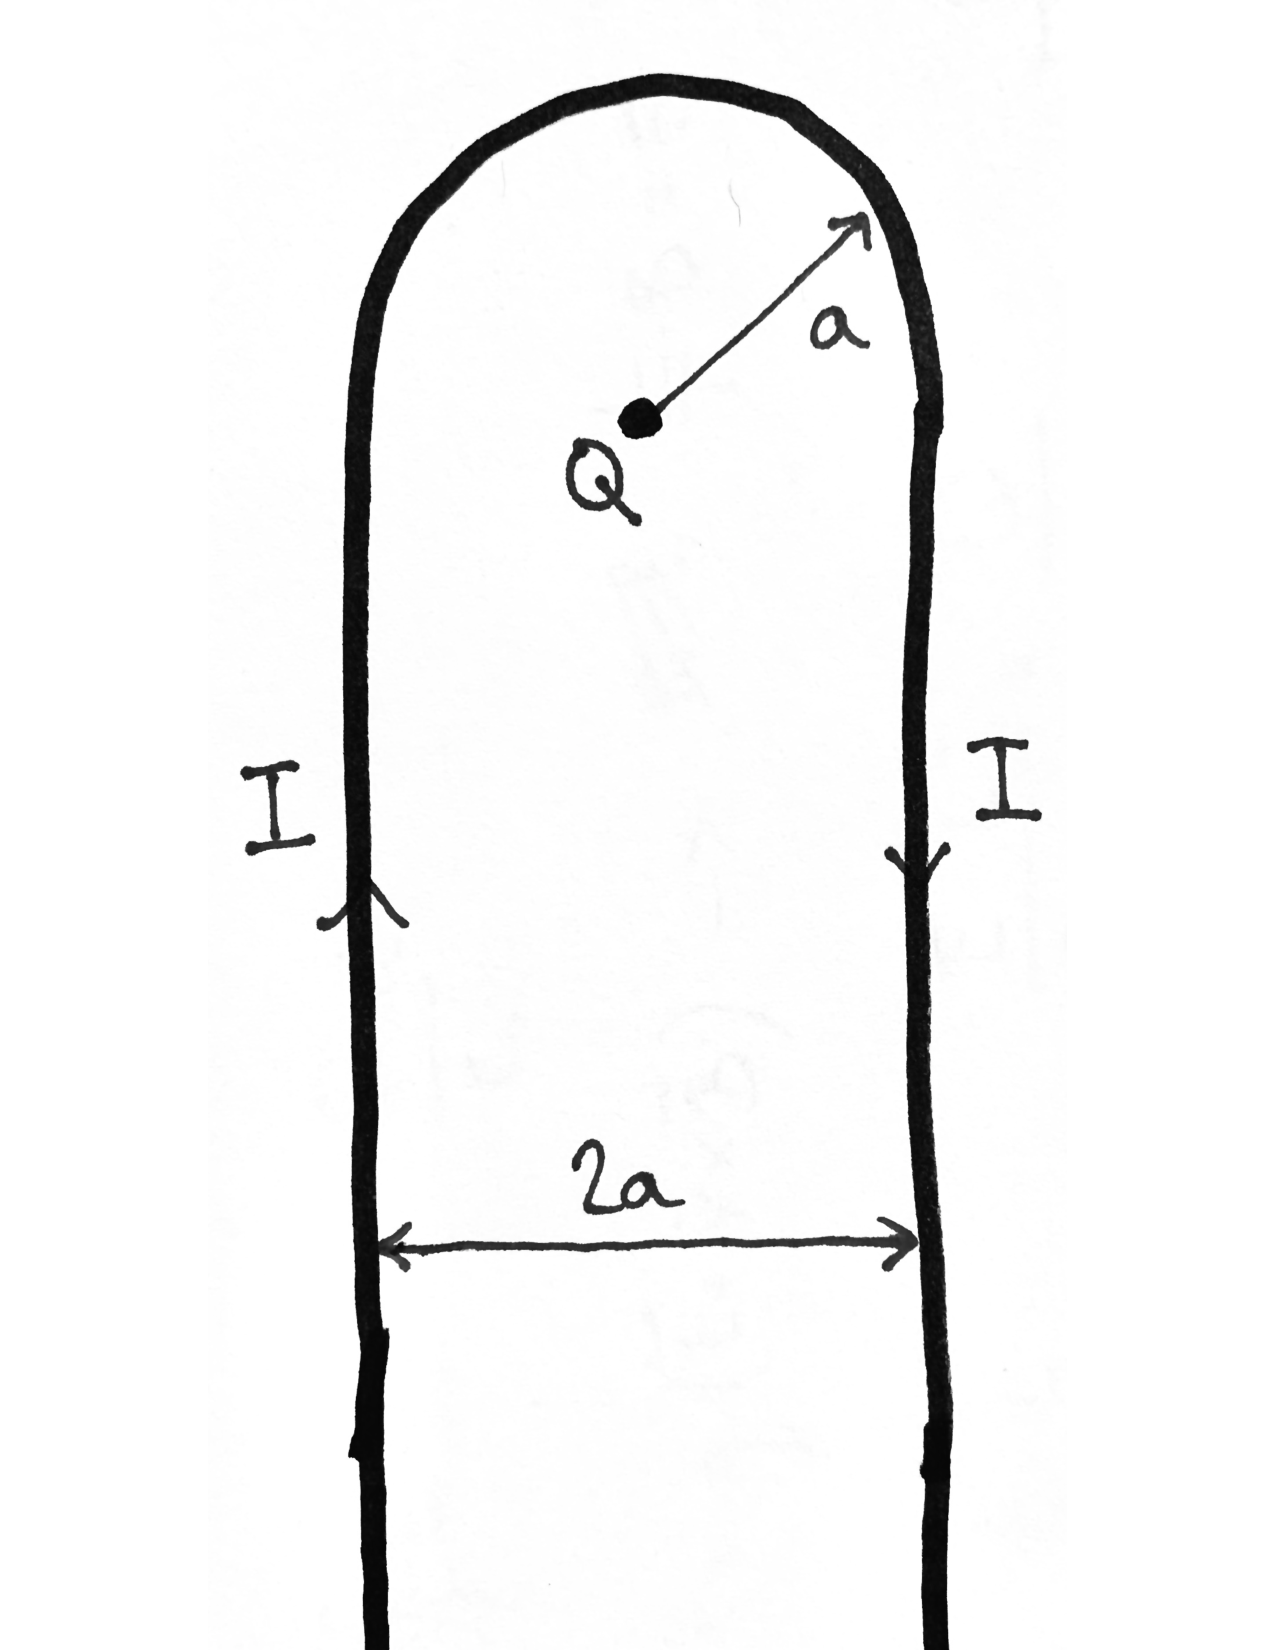
\includegraphics[width=\marginparwidth]{hairpin.pdf}}

\paragraph{Problem~\theproblem:}\refstepcounter{problem}%
Here's a terrible model for Earth's magnetic field: Imagine that
Earth's core is a circular current loop carrying current $I$, with
radius $R$ equal to the radius of the core. In this model, what does
the current have to be to make the field we observe at Earth's
north magnetic pole? Be as imprecise as you like. This is just an
order-of-magnitude problem! Give a numerical answer in Amperes.

\end{document}
